\section{Specification}

\subsection{Requirements} \label{ss:requirements}

\paragraph{Functional}

\begin{itemize}
  \item Log into their account
  \item View their saved account information
  \item View the jobs within their organisation
  \item View a job's assigned employees with their
        confirmed clock ins/outs
  \item View the verification chain for a job
  \item Clock in/out for their assignments
  \item Access a confirmation code for a job
\end{itemize}

\paragraph{Non-functional}
% TODO improve

In essence, the non-functional requirements are encompassed
by the \enquote{universal} guideline in the
\hyperref[s:motivation]{project motiviation}.

\subsection{Diagrams}

See Figures \ref{fig:erd}.

% TODO add architecture overview

\begin{figure}[H]
  \centering
  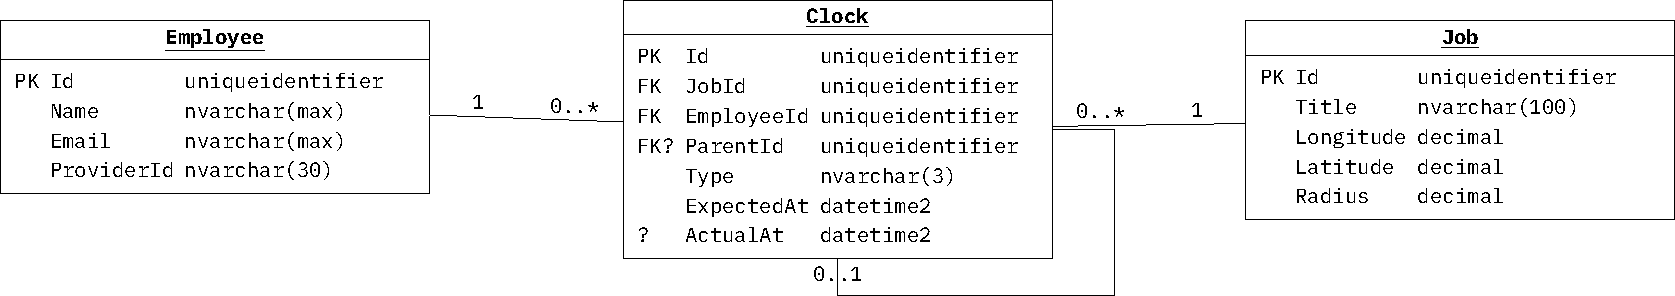
\includegraphics[width=\linewidth]
  {05 design/assets/entity relationship diagram.pdf}
  \caption{Entity Relationship Diagram}
  \label{fig:erd}
\end{figure}

\subsection{Epics} \label{ss:epics}

\newcommand{\epic}[2]
{
  \begin{tabular}{p{0.2\linewidth}p{0.8\linewidth}}
    \textbf{Title}       & #1 \\
    \textbf{Description} & #2 \\
  \end{tabular}
}

\epic{Initiation}
{
  The development and configuration of all subsystems to
  prepare the application for feature work.

  As this is a technical task, its user stories will not
  follow the \enquote{as a\ldots{} I want\ldots{} so
    that\ldots{}} template.
} \hline

\epic{Jobs}
{
  Functionality to interact with Jobs (e.g, viewing)
  plus directly associated data (e.g., assignments)
} \hline

\epic{Clocking}
{
  Functionality to implement the clocking feature: rules
  and user interface for location \& identity
  verification
}

\subsection{User Stories} \label{ss:stories}

\newcommand{\designs}[1]{\textbf{Designs} & Figures #1}

\newcommand{\story}[5]
{
  \begin{tabular}{p{0.2\linewidth}p{0.8\linewidth}}
    \textbf{Title}               & #1 \\
    \textbf{Epic}                & #2 \\
    \textbf{Description}         & #3 \\
    \textbf{Acceptance Criteria} & #4 \\
    #5
  \end{tabular}
}

\story{Backend Setup}{Initiation}
{
  Development and configuration of the API
}
{
  Ready to implement business functionality
}{} \hrule

\story{Frontend Setup}{Initiation}
{
Development and configuration of the web client
}
{
\begin{itemize}[leftmargin=*]
  \item Ready to implement business functionality
  \item Able to send requests and handles responses with
        the API
\end{itemize}
}{} \hrule

\story{Authentication}{Initiation}
{
As a user, I want to log into the application, so that
I can use its services
}
{
\begin{itemize}[leftmargin=*]
  \item The frontend displays a page to login when opened
  \item Users can login via Auth0 using social providers
  \item API routes and web pages which require auth cannot
        be accessed without logging in
  \item New user details are persisted in the database
\end{itemize}
}
{
\designs{\ref{fig:homePageNoAuth},
  \ref{fig:homePageWithAuth}}
} \hrule

\story{Viewing Jobs}{Jobs}
{
  As a user, I want to view jobs, so that I can get their
  information and clock in/out
}
{
  \begin{itemize}[leftmargin=*]
    \item Users can view the jobs in the system, showing
          its principle details
    \item Viewing a Job individually shows the employees
          assigned
  \end{itemize}
}
{
  \designs{\ref{fig:jobsPage}, \ref{fig:jobPage}}
} \hrule

\story{Providing Location}{Confirmation}
{
  As an employee, I want to provide my location to submit
  a clock
}
{
  In all cases:
  \begin{itemize}
    \item Location must be within the radius of the job
    \item Can only clock in/out of their own job
  \end{itemize}

  When clocking in:
  \begin{itemize}
    \item Job cannot have ended
    \item Cannot currently be clocked in
    \item Cannot have clocked out
    \item Cannot clock in too early for a job
  \end{itemize}

  When clocking out:
  \begin{itemize}
    \item Cannot already be clocked out
    \item Must be currently clocked in
    \item Cannot clock out too late
  \end{itemize}
}
{
  \designs{\ref{fig:jobPage}, \ref{fig:clockPage}}
} \hrule

\story{Confirming Location \& Identity}{Confirmation}
{
  As an employee, I want to confirm my clock, so that I can
  prove the clock was not performed by another employee
}
{
  See the base criteria in \enquote{Providing Location}

  \begin{itemize}
    \item The first employee does not need to confirm the
          clock in (principle verifier)
    \item All subsequent employees are required to confirm
          their clocks
    \item All subsequent employees can only confirm via a
          confirmed employee
    \item Confirmation codes should be limited to a single
          employee and a predetermined lifetime
    \item When clocking, information about the confirmed
          employees should be available
    \item Jobs with one assigned employee require no
          confirmation
  \end{itemize}
}
{
  \designs{\ref{fig:clockPage}, \ref{fig:confirmPage}}
} \hrule

\story{Viewing Verification Chain}{Confirmation}
{
  As a user, I want to view the verification chain, so that
  I can review the clock ins/outs visually
}
{
  Each job has a diagram displaying its clock ins and outs
}
{
  \designs{\ref{fig:confirmationsPage}}
}
